\chapter{Part III: The Art of Listening}

This chapter follows the movement of a dialogue between J. Krishnamurti and Dr. Alan W. Anderson on seeing, hearing, learning, attention, and freedom. There is no blackboard mathematics here in the usual sense. The structure is nevertheless exacting: Krishnamurti is asking us to distinguish direct perception from perception mediated by memory, image, belief, and reward. We will keep the order of the inquiry and use a little formal notation only as a bookkeeping device, never as a substitute for the spoken investigation.

\section{The Question of Seeing}

The dialogue begins by taking up a promise from the previous conversation. They had been speaking about beauty and transformation, and the unresolved question was seeing: whether seeing can be independent of knowledge and time. Krishnamurti immediately refuses to treat seeing as a merely optical event. The question is not whether the eye receives light. The question is whether the mind actually sees.

Let us mark the object perceived by \(O\), the perceiving mind by \(M\), and the intervening screens by \(S_1,S_2,\ldots,S_n\). This notation is only a reconstruction of the inquiry, but it helps us keep the structure in view:
\begin{equation}
M \xrightarrow{\;S_1,S_2,\ldots,S_n\;} O .
\end{equation}
The point of the formula is not that perception is a mechanical pipeline. The point is that the ordinary mind rarely meets the thing directly. It meets it through prejudice, idiosyncrasy, experience, wishes, pleasures, fears, images, beliefs, and memories.

\begin{definition}
In this chapter, a \emph{screen} means any image, memory, belief, fear, pleasure, or conclusion through which perception is filtered before the thing itself is met.
\end{definition}

Krishnamurti's first pressure is therefore very simple: if these screens stand between us and the object, do we ever see the thing at all? Seeing may not take place. What we call seeing may be recognition, naming, comparison, expectation, or the operation of memory.

\begin{figure}
\centering
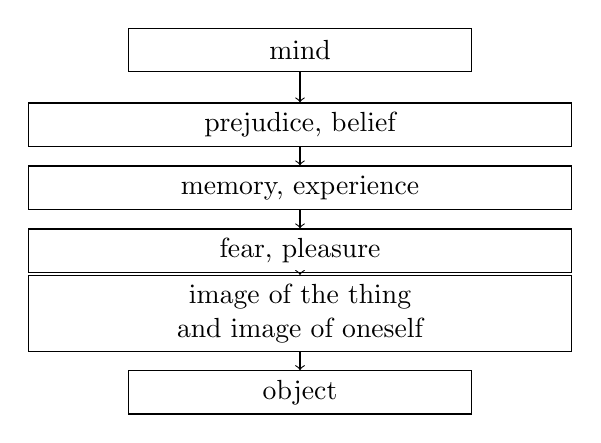
\begin{tikzpicture}
\node[draw, align=center, text width=0.34\linewidth, minimum height=0.55cm] (mind) at (0,4.2) {mind};
\node[draw, align=center, text width=0.55\linewidth, minimum height=0.55cm] (s1) at (0,3.25) {prejudice, belief};
\node[draw, align=center, text width=0.55\linewidth, minimum height=0.55cm] (s2) at (0,2.45) {memory, experience};
\node[draw, align=center, text width=0.55\linewidth, minimum height=0.55cm] (s3) at (0,1.65) {fear, pleasure};
\node[draw, align=center, text width=0.55\linewidth, minimum height=0.55cm] (s4) at (0,0.85) {image of the thing\\and image of oneself};
\node[draw, align=center, text width=0.34\linewidth, minimum height=0.55cm] (object) at (0,-0.15) {object};
\draw[->] (mind) -- (s1);
\draw[->] (s1) -- (s2);
\draw[->] (s2) -- (s3);
\draw[->] (s3) -- (s4);
\draw[->] (s4) -- (object);
\end{tikzpicture}
\caption{A reconstructed map of Krishnamurti's ``screen after screen'' account of perception.}
\end{figure}

The important turn is the question whether the mind can look without those screens. This is not a method yet. It is not practice, not discipline, not a technique. It is the first form of the whole inquiry: can the mind look without image, conclusion, belief, memory, prejudice, and fear?

\section{Seeing and Action}

Once seeing is raised, action appears immediately. This is one of the decisive moves in the dialogue. Krishnamurti says that when there is a seeing of the thing, there is no question of postponement, succession, or interval. We may write the structural claim as
\begin{equation}
\hbox{direct seeing} \Rightarrow \hbox{action without interval}.
\end{equation}
This should not be read as a psychological law in the modern technical sense. It is a way of preserving the lecture's distinction: direct perception is not followed by a separate deliberative process in which an idea is selected and then implemented.

The contrast is action based on belief, conclusion, or idea:
\begin{equation}
\hbox{belief/conclusion/idea}
\Rightarrow
\hbox{time-binding action}
\Rightarrow
\hbox{conflict, sorrow, regret}.
\end{equation}
Here ``time-binding'' means action bound to postponement, succession, interval, and consequence. The mind acts from a formula; the formula belongs to the past; therefore the action carries the past forward.

\subsection{Question \& Answer}

\paragraph{Question.}
If action is not based on an idea, how does action occur?

\paragraph{Answer.}
In the structure of this dialogue, the answer is that action is not separated from seeing. If the danger, falseness, or fact is seen directly, action is already implied in that seeing. The interval appears only when seeing has been replaced by belief, conclusion, or formula. Anderson later phrases this as one act: the action and the seeing are not two separate operations.

A compact way to record the distinction is:
\begin{align}
\hbox{direct seeing} &\Rightarrow \hbox{no interval},\\
\hbox{idea-based action} &\Rightarrow \hbox{interval and conflict}.
\end{align}

This is why the chapter must not treat seeing as a preliminary topic and action as a later moral application. In the lecture, the two are already bound together.

\section{Listening Without Interference}

From seeing, Krishnamurti turns to hearing. The same structure returns, now in relationship. We may hear a wife, husband, girl, boy, or friend through the image built about that person. We hear through irritation, annoyance, domination, conclusion, and the accumulated history of relationship. The question becomes: do we ever hear another directly?

Anderson recalls an earlier remark: hearing is doing nothing to stop or interfere with seeing. That is an important bridge. Hearing is usually imagined as effort: ``hear me out,'' lean forward, concentrate, obey the command. But Krishnamurti is moving in the opposite direction. Listening is not the tightening of effort; it is the absence of interference.

Let \(L\) denote listening and \(I\) denote interference: translation, interpretation, conclusion, comparison, like and dislike. The reconstructed relation is
\begin{equation}
L_{\rm direct}=L-I .
\end{equation}
The notation is deliberately simple. It does not claim that listening is a measurable quantity. It says that the lecture's operational distinction is subtractive: listening is not produced by adding strain; it appears when interference is absent.

The next step is sharper. Krishnamurti asks what takes place when one actually listens to a statement. This is the local place where the dialogue becomes almost procedural.

\section{The Abstraction Loop}

The example is a statement about beauty, passion, and sorrow. The ordinary mind hears the words, draws a conclusion, forms an idea, and then asks how to carry out that idea. At that moment the statement has become a problem.

The sequence can be written as a reconstructed update rule:
\begin{equation}
\hbox{statement}
\to
\hbox{words}
\to
\hbox{conclusion}
\to
\hbox{idea}
\to
\hbox{problem of implementation}.
\end{equation}
This is one of the cleanest structures in the lecture. The mind converts hearing into abstraction, and abstraction into a project. Once a statement has become an idea, different minds carry different ideas and clash over embodiment.

\begin{proposition}
If a statement is converted into an idea, the mind no longer listens to the statement directly; it deals with its own abstraction.
\end{proposition}

\begin{proof}
The transcript gives the steps. First, the statement is heard as words. Second, the mind draws a conclusion from those words. Third, that conclusion becomes an idea. Fourth, the mind asks how to carry out the idea. The practical problem belongs not to the original listening, but to the abstraction formed from it. Therefore the mind is now acting on its own construction rather than listening directly.
\end{proof}

\subsection{Question \& Answer}

\paragraph{Question.}
What happens when a statement is heard without abstraction?

\paragraph{Answer.}
Krishnamurti's answer is not that the mind arrives at a better conclusion. It does not compare, agree, disagree, or form an idea. It listens. In that listening there is attention, and in attention the truth or falseness of the statement is seen in the very act of hearing it.

The distinction may be recorded as:
\begin{align}
\hbox{ordinary hearing}
&:\quad
\hbox{statement}\to\hbox{idea}\to\hbox{problem},\\
\hbox{complete listening}
&:\quad
\hbox{statement}\to\hbox{attention}.
\end{align}
The second line is not an instruction to simplify thought. It is the lecture's claim that total attention does not need the detour through abstraction.

\section{Attention Without Reward}

The dialogue now opens into the question of attention. Krishnamurti says that attention means no border. The moment attention has a frontier, concepts arise; then agreement, disagreement, resistance, and conflict begin.

We can formulate the border condition schematically:
\begin{equation}
\hbox{frontier in attention}
\Rightarrow
\hbox{concept, comparison, conflict}.
\end{equation}
The absence of frontier is not a blank state. It is total attention. Because there is no border from which the mind stands apart and judges, the mind is free to act.

Anderson then gives a personal example from the conversations themselves: intense listening has not divided his mind from the practical necessities of being filmed. Krishnamurti's response moves the inquiry into reward. Our minds, he says, are commercial. We want exchange: I give this, I receive that. We torture ourselves religiously, and God must come to us. The same structure appears when people ask how to maintain attention.

The false maintenance question can be written:
\begin{equation}
\hbox{practice attention}
\to
\hbox{obtain reward}.
\end{equation}
But this belongs to the very commerce the dialogue is exposing. Krishnamurti says attention is not a result and has no cause. What has a cause has an effect, and the effect becomes the cause. That circular movement can be represented as:
\begin{figure}
\centering
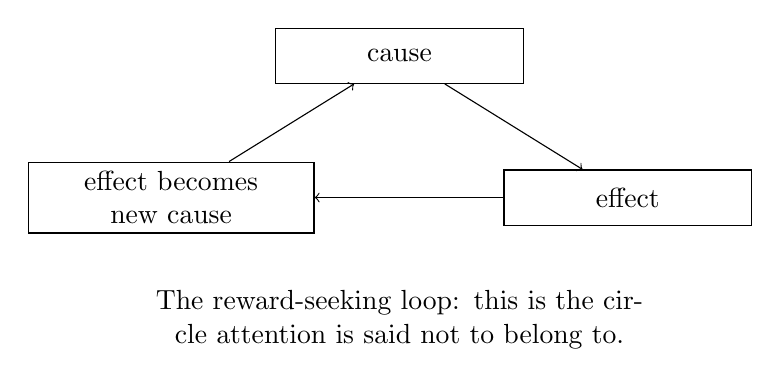
\begin{tikzpicture}
\node[draw, align=center, text width=0.24\linewidth, minimum height=0.7cm] (cause) at (0,2.2) {cause};
\node[draw, align=center, text width=0.24\linewidth, minimum height=0.7cm] (effect) at (2.9,0.4) {effect};
\node[draw, align=center, text width=0.28\linewidth, minimum height=0.7cm] (newcause) at (-2.9,0.4) {effect becomes\\new cause};
\draw[->] (cause) -- (effect);
\draw[->] (effect) -- (newcause);
\draw[->] (newcause) -- (cause);
\node[align=center, text width=0.58\linewidth] at (0,-1.15) {The reward-seeking loop: this is the circle attention is said not to belong to.};
\end{tikzpicture}
\caption{A reconstructed diagram of the cause-effect circle discussed in relation to reward and attention.}
\end{figure}

Thus the question ``How shall I maintain attention?'' is already the wrong question. It turns attention into an object of acquisition. It asks for a method that will guarantee a return.

\section{Learning and the Mechanical Mind}

At this point the lecture pivots. Seeing and hearing have led to learning because they are not separate chapters. They are one movement. Krishnamurti asks whether learning is accumulation, and whether there is any other learning.

The first kind of learning is obvious and necessary: learning a language, learning to ride a bicycle, learning to drive a car, learning a craft, learning a livelihood. This is the acquisition of knowledge in action. Let us call this \(K_{\rm mech}\), mechanical knowledge:
\begin{equation}
\hbox{experience}+\hbox{knowledge}
\to
\hbox{memory}
\to
K_{\rm mech}
\to
\hbox{routine action}.
\end{equation}
The important caution is that Krishnamurti does not dismiss this. In its field it is necessary. The question is whether this is the only learning.

\begin{definition}
\emph{Mechanical learning} is learning as accumulation: experience stored as memory and used as skill, routine, profession, or practical function.
\end{definition}

The inquiry becomes more disturbing when it reaches experience. We often say, ``I have learned from experience.'' Krishnamurti asks whether we have. Human beings have had wars, sorrow, uncertainty, suffering, and violence across history. If experience were enough, repetition would have ended. But repetition continues.

The test is:
\begin{align}
\hbox{repeated experience of sorrow}
&\not\Rightarrow
\hbox{freedom from sorrow},\\
\hbox{repeated experience of war}
&\not\Rightarrow
\hbox{freedom from war}.
\end{align}
So in the deeper sense under investigation, one has learned nothing except in the field of knowledge. The mind remains mechanical: repetitive reactions, repetitive demands, repetitive pursuits. Thought is always old; there is no new thought in the movement of the known.

The phrase ``known to known'' can be recorded as:
\begin{equation}
\hbox{known}\to\hbox{known}
\Rightarrow
\hbox{movement in time}
\Rightarrow
\hbox{not freedom}.
\end{equation}

\subsection{Question \& Answer}

\paragraph{Question.}
Is there any non-mechanical learning?

\paragraph{Answer.}
The dialogue does not answer by adding a second category of learning to the first. Krishnamurti pushes the question until the very notion of psychological accumulation is exposed. One can learn a language or a craft. One can learn about oneself as the known, because the self is accumulated knowledge of the past. But to learn about God, freedom, or the inward as if these were new objects of accumulation is to continue the same mechanical movement.

This is why the question becomes: if there is no other learning in the accumulative sense, what takes place? The answer is not another subject to learn, but the understanding of the movement of knowledge itself.

\section{Knowledge, Silence, and Meditation Deferred}

The later part of the dialogue asks what happens when the mind understands the whole field of knowledge. Anderson brings in Vedanta as the end of knowledge, and Krishnamurti keeps the point practical: the mind knows the activity of the known. What is the state of the mind that is free from that and yet functions in knowledge?

This is the deepest apparent contradiction in the lecture. Freedom is not ignorance, and functioning in knowledge is not the same as being bound by knowledge. The distinction can be recorded as:
\begin{equation}
\hbox{functioning in knowledge}
\neq
\hbox{psychological bondage to knowledge}.
\end{equation}
The mind must function in practical knowledge. We could not speak, drive, build, teach, or carry out ordinary tasks without it. But when knowledge occupies the whole field, seeing and listening become mechanical. The flower is never new; it is recognized as the expected rose. Perception moves from known to known.

Krishnamurti then asks whether there is a listening out of silence. In that silence, there is no demand, no reward, no punishment, no project of self-improvement. He identifies that listening with attention:
\begin{equation}
\hbox{silence}+\hbox{listening}
\Rightarrow
\hbox{attention not bound to time}.
\end{equation}
Anderson notices that meditation, in this sense, is not something done in succession. Krishnamurti refuses to expand the topic fully here. He says meditation must be gone into deeply another time, partly because the word has been damaged by technique, scheduling, payment, and the notion of learning meditation as another acquisition.

The recap is crucial. The dialogue began with beauty, then passion, suffering, action, seeing, and hearing. It then exposed mechanical seeing and mechanical listening, the known-to-known movement, and the falseness of freedom when freedom is only an idea. The final question is whether one can observe out of silence and still act in the field of knowledge, both together in harmony.

\section{Words and the Thing}

Before the dialogue closes, Anderson offers an example from teaching: students may think about a doctrine, but hesitate when asked to look directly. Krishnamurti draws the lesson back to words. We are caught in words; the word is not the thing, but the description often becomes all that matters.

This belongs exactly to the earlier structure of screens. The word becomes another screen:
\begin{equation}
\hbox{word} \neq \hbox{thing}.
\end{equation}
When the word becomes important, the door named by the word disappears behind the name. Education often strengthens this abstraction. Philosophy may theorize endlessly about how one should live while not living it.

The movement is now visible:
\begin{align}
\hbox{thing}
&\to
\hbox{word}
\to
\hbox{abstraction}
\to
\hbox{theory},\\
\hbox{direct seeing}
&\to
\hbox{appropriate action}.
\end{align}
This is why the chapter should not end in concept. The lecture's pressure is toward seeing, listening, and acting without the detour through abstraction.

\section{Summary}

The art of listening, in this dialogue, is not a technique for becoming a better listener. It is part of a single inquiry into seeing, hearing, learning, action, knowledge, and freedom. Seeing through screens is not seeing. Hearing through image and conclusion is not listening. Action based on idea is time-binding. Attention is not produced by cause, reward, or practice. Mechanical learning is necessary in its field, but it does not answer the deeper question of freedom.

The chapter's central map is therefore:
\begin{equation}
\hbox{screens}
\to
\hbox{abstraction}
\to
\hbox{time-binding action}
\to
\hbox{conflict},
\end{equation}
and its counter-movement is:
\begin{equation}
\hbox{silence}
\to
\hbox{attention}
\to
\hbox{direct seeing/listening}
\to
\hbox{action without interval}.
\end{equation}
These equations are not formal psychology. They are compact reminders of the lecture's order. Krishnamurti begins with perception and ends at the edge of meditation, but he does not let meditation become a method. He leaves us with a more exacting question: can the mind understand the movement of knowledge, observe out of silence, and act in the field of knowledge without being bound by it?